\documentclass{../source/Experiment}

\major{信息工程}
\name{}
\title{回归模型}
\stuid{}
\college{信息与电子工程学院}
\date{\today}
\lab{教11-400}
\course{人工智能实验}
\instructor{胡浩基、魏准}
\grades{}
\expname{回归模型}
\exptype{设计验证}
\partner{}
\begin{document}
\makecover
\section{实验题目}
\subsection{线性回归}
编写程序,通过产生的附加噪声的随机数据,(1)做线性回归(即求出𝜽);(2)利用取得的回归模型,对x=0和x=2两个点做预测;(3)对上述随机数据和预测结果利用plot可视化。

\subsection{多项式回归}

通过网上调研了解Scikit -Learn中的LinearRegression模块,编写程序,利用LinearRegression模块:(1)对上述产生的二级多项式数据(X\_poly, y) 做线性回归。(2) 可视化回归模型和数据。


\subsection{逻辑回归}

(1)查阅网上资料,通过sklearn.linear\_model中的LogisticRegression,利用花瓣宽度,实现一个分类器检测维吉亚鸢尾花。
(2)可视化花瓣宽度0-3 cm之间的鸢尾花模型估算出的概率

\section{实验代码}
\subsection{线性回归}
\lstinputlisting[
    language  =   Python,
    title = {Linear Regression}
]{./Part2/lab1.py}
\lstinputlisting[
    language  =   Python,
    title = {Polynomial Regression}
]{./Part1/lab2.py}
\subsection{多项式回归}
\lstinputlisting[
    language  =   Python,
    title = {Logistic Regression}
]{./Part2/lab3.py}
\subsection{多项式回归}

\section{实验结果}
\subsection{线性回归}

结果如下:

θ = [4.122495, 2.863779]

模型为:
$$ y = 4.122495 + 2.863779x$$
预测情况:

x = 0 , y = 4.122495

x = 2 , y = 9.850053


结果可视化如下图:
\begin{figure}[H]
    \centering
    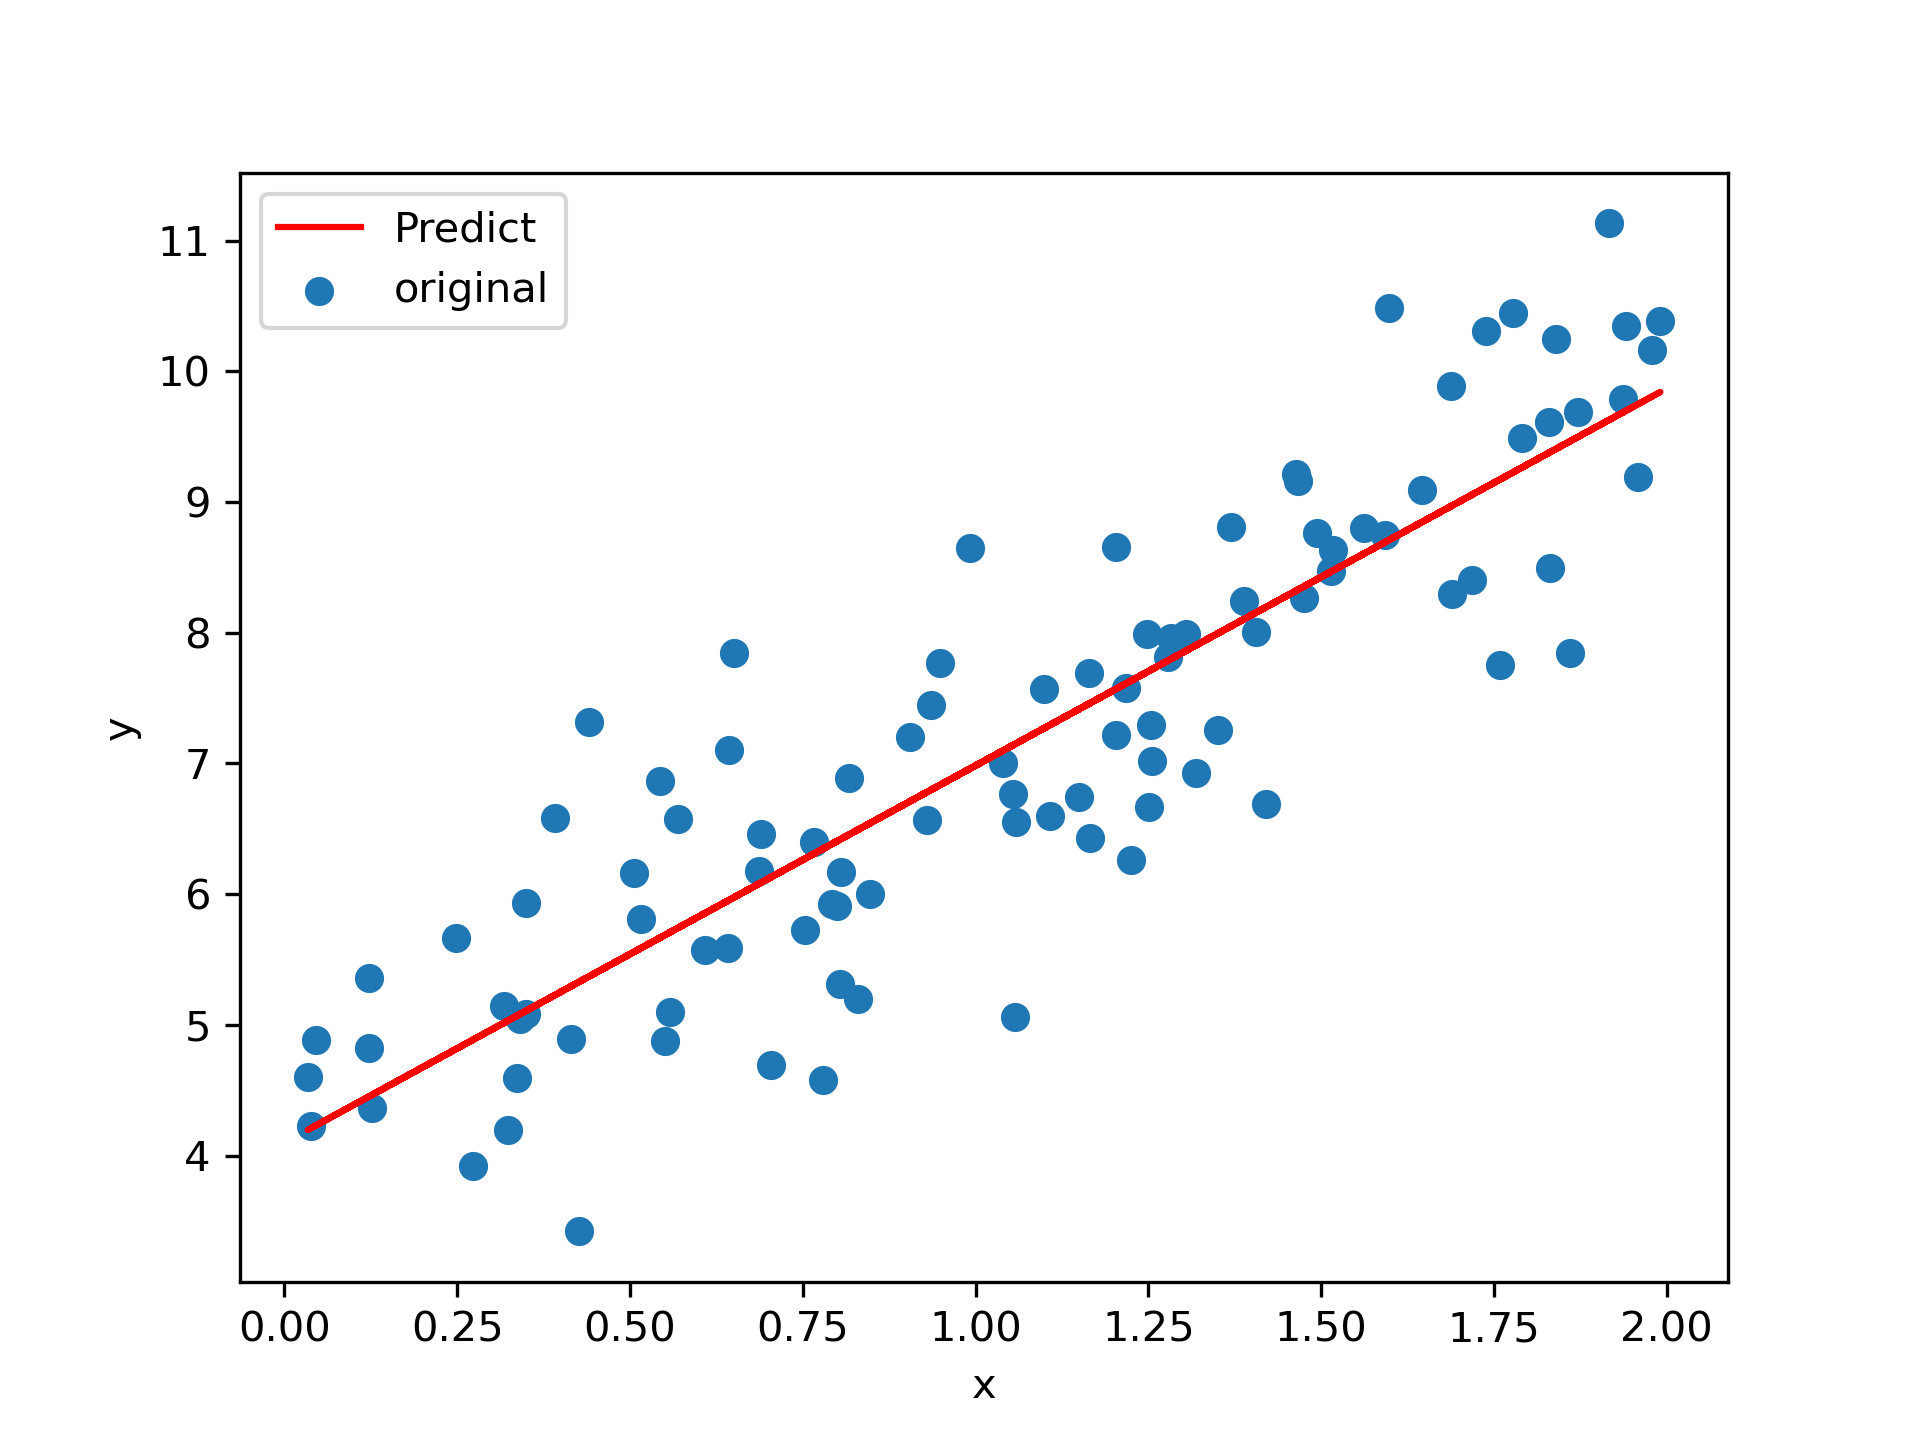
\includegraphics[width = 0.6\textwidth]{Part2/figure1.png}
    \caption{线性回归结果可视化}
\end{figure}

\subsection{多项式回归}
结果如下:

系数 = [0.94986314, \, 0.47823706]

截距 = [2.03896946]

模型为:
$$ y = 0.47823706x^2 + 0.94986314x + 2.03896946$$

结果可视化如下图:
\begin{figure}[H]
    \centering
    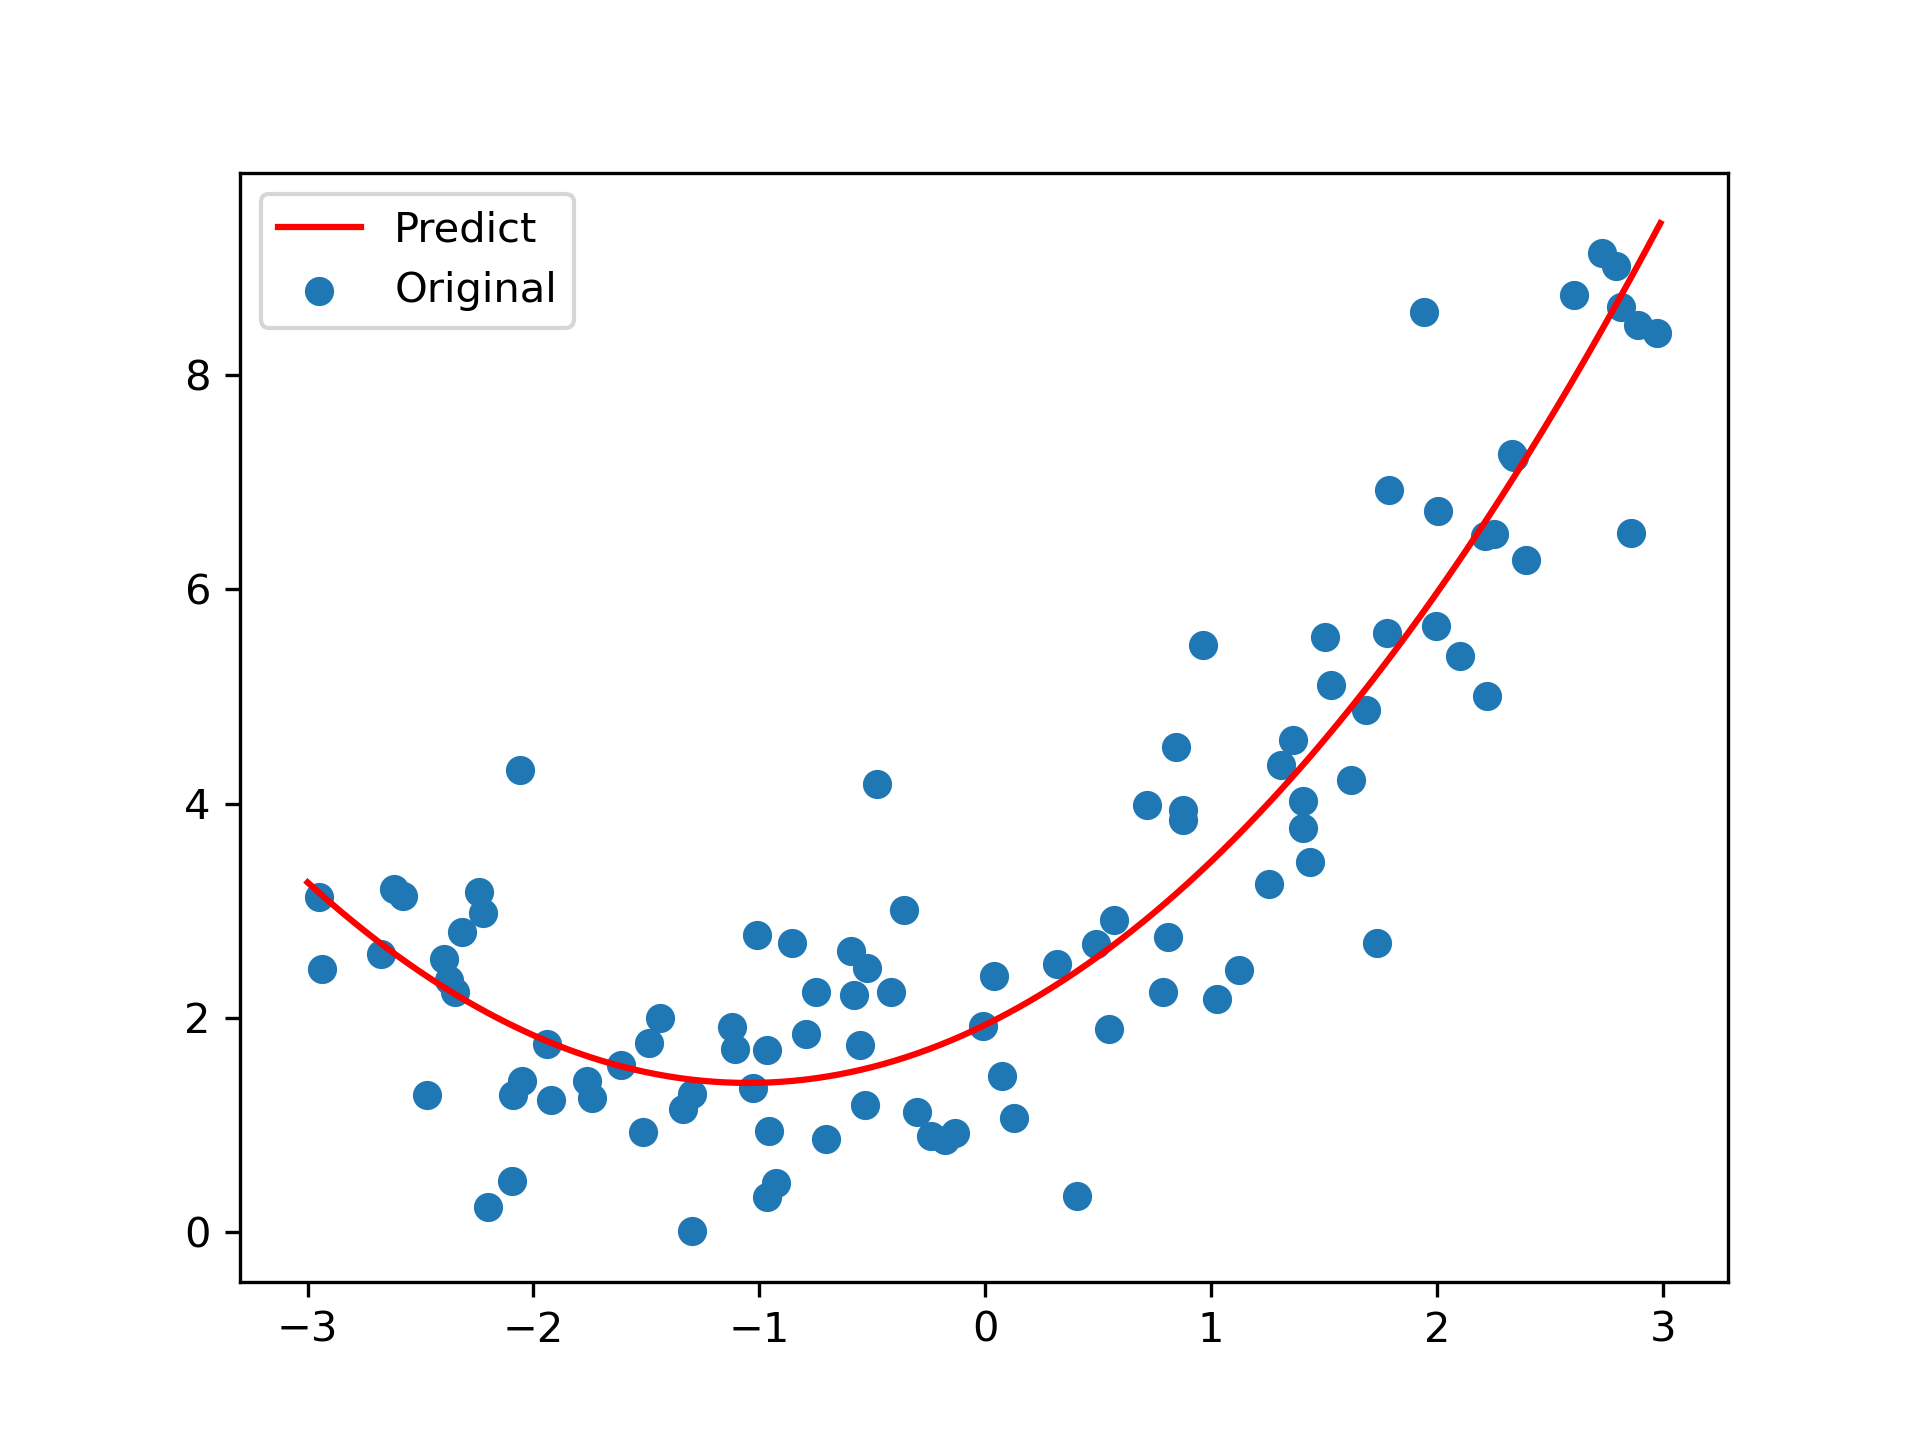
\includegraphics[width = 0.6\textwidth]{Part2/figure2.png}
    \caption{多项式回归结果可视化}
\end{figure}
\subsection{逻辑回归}

结果可视化如下图:
\begin{figure}[H]
    \centering
    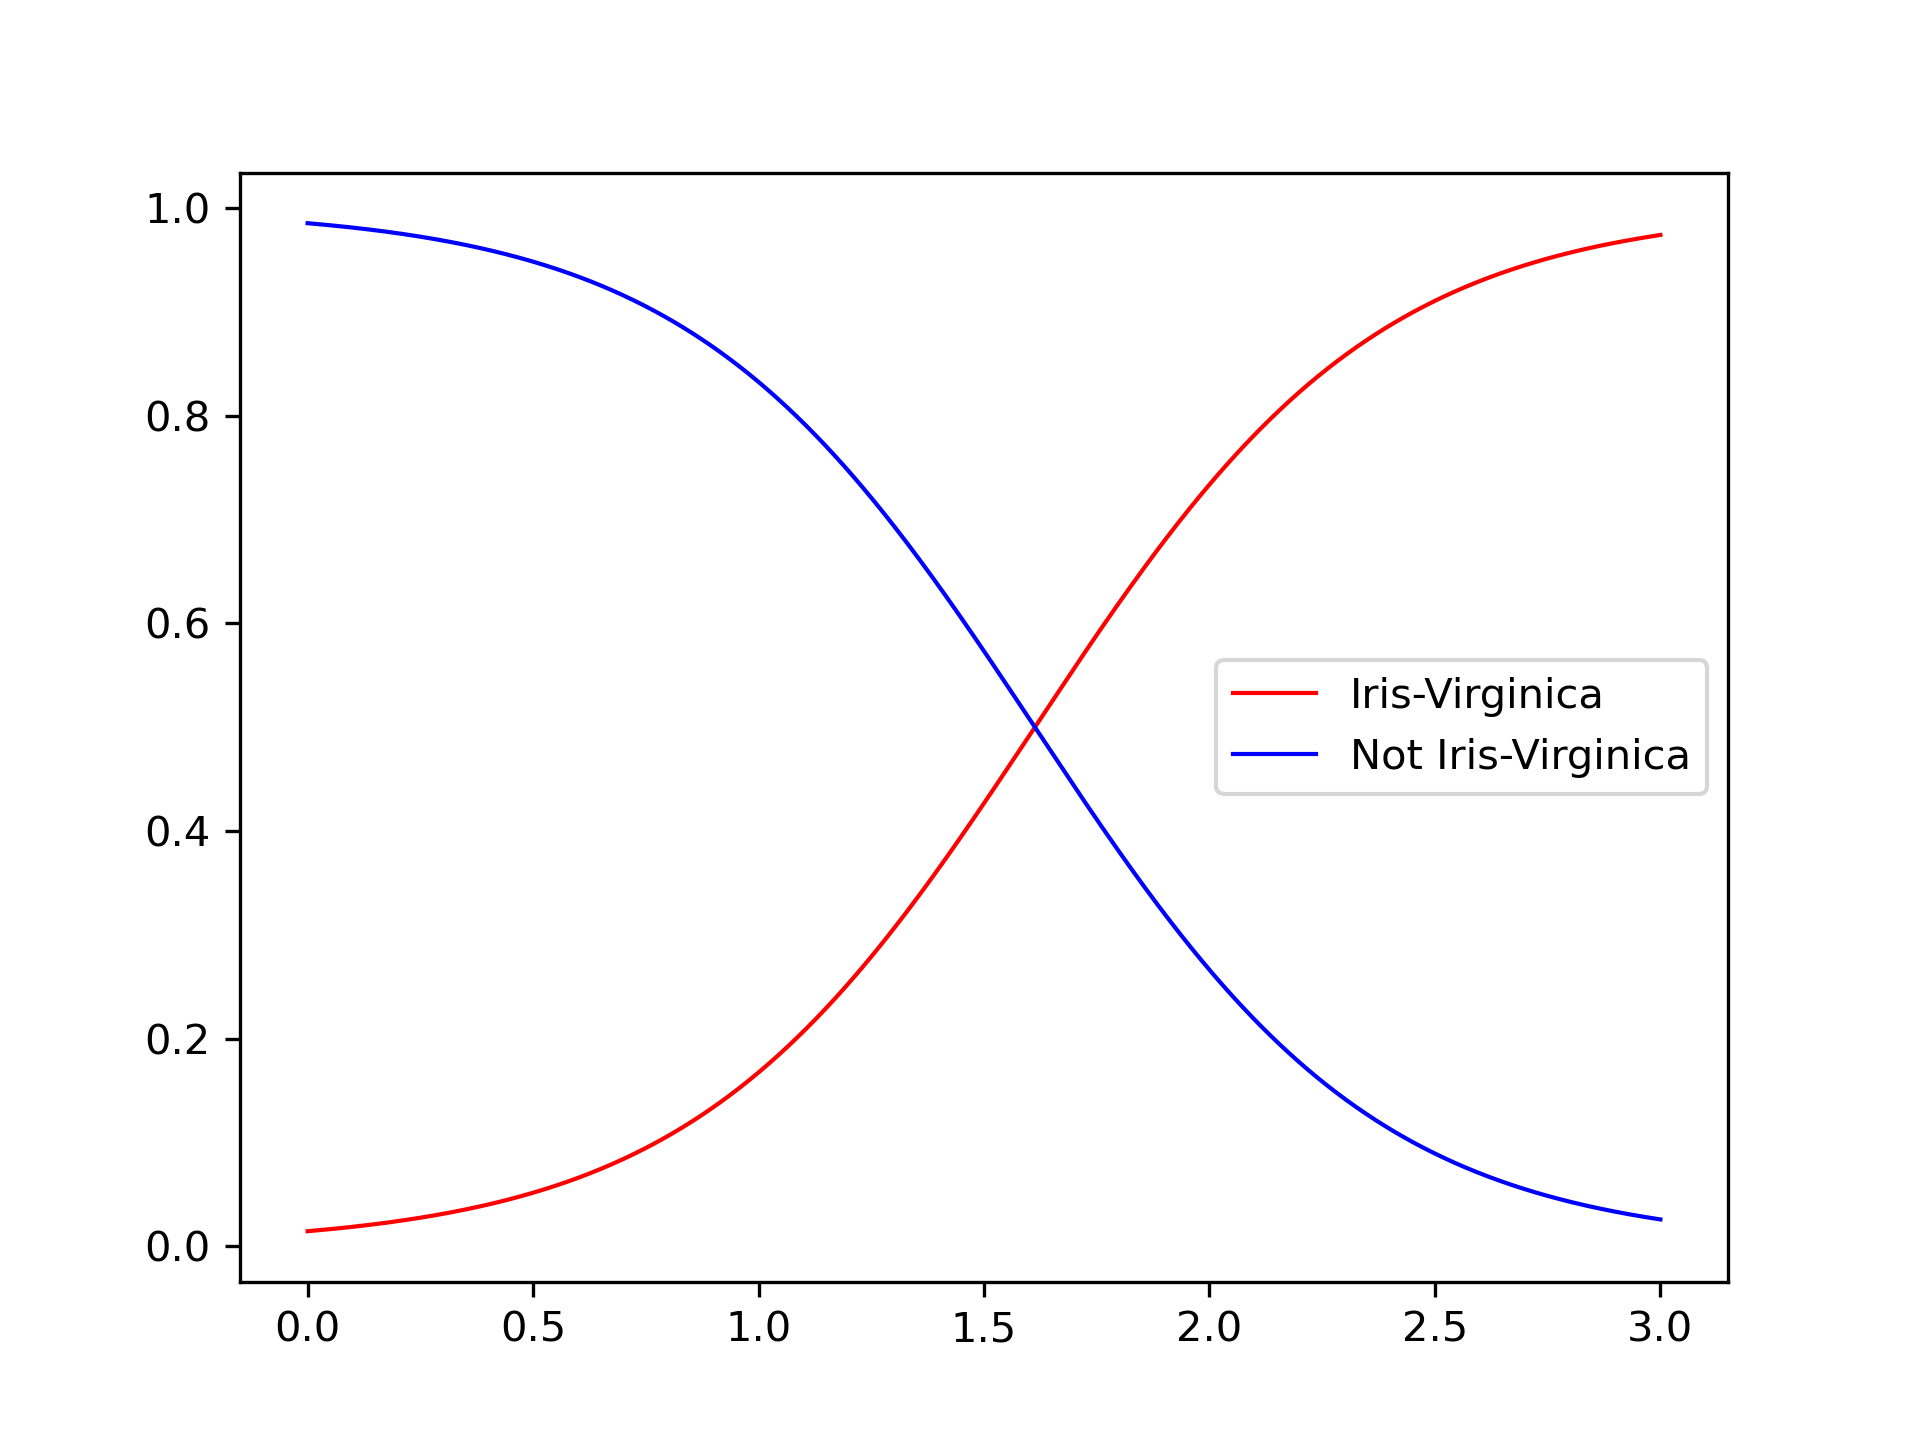
\includegraphics[width = 0.6\textwidth]{Part2/figure3.png}
    \caption{逻辑回归结果可视化}
\end{figure}
\end{document}


